% F27 KD temperature sweep plot (exp9). Added 6 Nov. RESULTS PENDING.
% When the sweep is done, scripts/analysis/kd_temperature_sweep.py writes
% results/experiments/exp9_kd_temperature/kd_temperature_sweep.pdf (x = temperature, log2; y = error in mm; one line
% per metric and dataset; teacher PVE dashed, 95% bars dotted; the reported T 4 run as its own marker). Copy it here:
%   cp results/experiments/exp9_kd_temperature/kd_temperature_sweep.pdf docs/thesis/figures/img/F27_kd_temperature.pdf
% Until then the figure shows a framed "pending" box, so the build never breaks.
\begin{figure}[!tbp]
\centering
\IfFileExists{figures/img/F27_kd_temperature.pdf}{%
  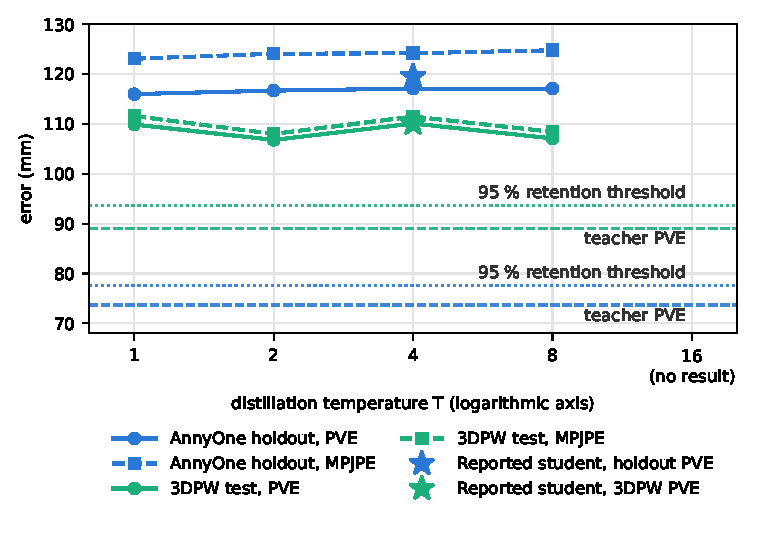
\includegraphics[width=0.8\linewidth]{F27_kd_temperature.pdf}%
}{%
  \fbox{\parbox[c][5cm][c]{0.75\linewidth}{\centering
    \TODO{figure pending}\\[1ex]
    \small KD temperature sweep, $T \in \{1, 2, 4, 8, \KDSweepMaxT\}$: error against temperature.\\
    Copy \texttt{kd\_temperature\_sweep.pdf} to \texttt{figures/img/F27\_kd\_temperature.pdf}.}}%
}
\caption[Distillation temperature sweep (plot)]{Student error against the feature-distillation temperature $T$
(logarithmic axis): PVE, PA-PVE and MPJPE on the AnnyOne holdout (V1) and on the 3DPW test set. Dashed lines: the
teacher's PVE (\FinalPVE{} and \FinalThreeDPW\,mm); dotted lines: the 95\,\% bars (\BarPVE{} and \BarThreeDPW\,mm);
separate marker: the reported $T = \MethodKDTemp$ run. Numbers in Table~\ref{tab:kd-temperature}.}
\label{fig:kd-temperature}
\end{figure}
